\chapter{Character Theory}
\thispagestyle{empty}

\begin{wrapfigure}[2]{r}{0.45\linewidth}
    \vspace{-15em}
    \centering
    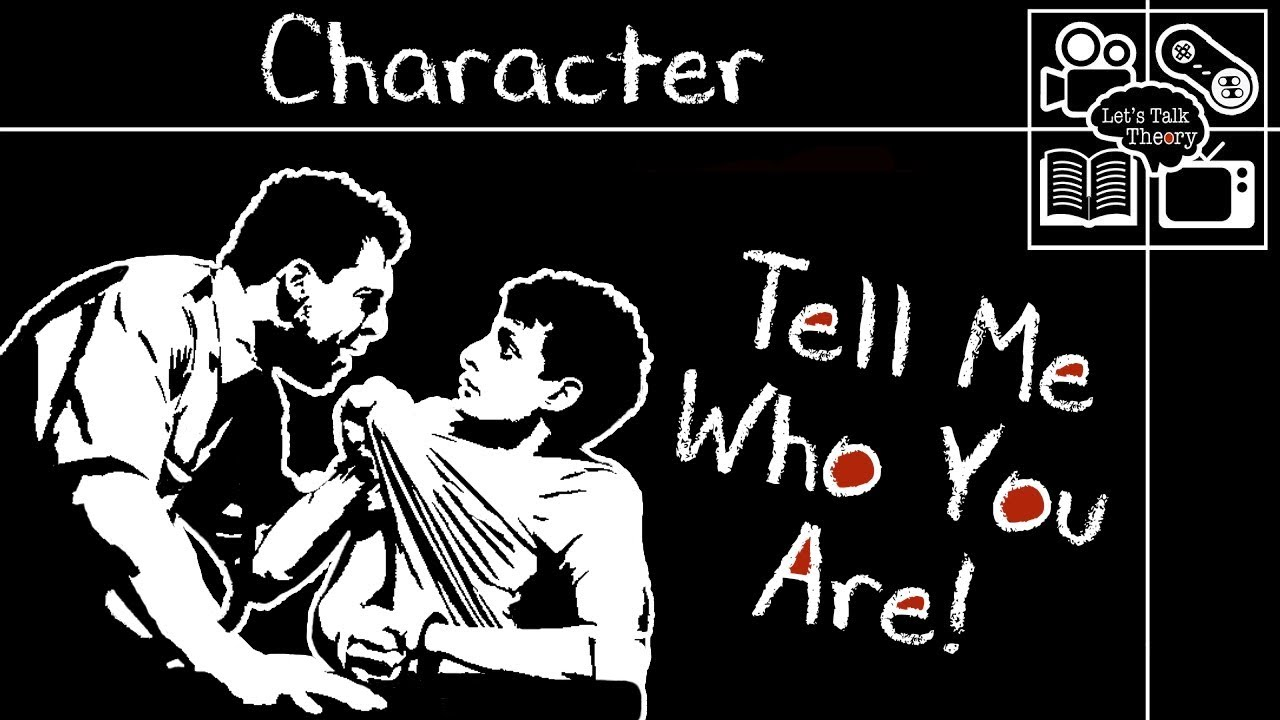
\includegraphics[width=0.8\linewidth]{./Chapters/2_Char/IMG_Char_Thy.jpg}
    \caption{\centering \small The thumbnail of a YouTube video titled ``What is Character Theory? $\vert$ Let's Talk Theory" by Dapper Mr. Tom. The video has nothing to do with mathematics.}
\end{wrapfigure}

In this chapter, we study an important type of functions from groups to fields known as characters. As we shall see, characters encode several useful properties of a group, and have been used extensively to prove several results about finite groups, (the representations of) which are the main object of study in this course. One of the reasons characters are useful to understand representation structures is that they are \textit{class functions}. That is, they encode information not about an individual element of a group but about its conjugacy class, making them good indicators of \textit{structural} and \textit{behavioural} properties. In particular, the character of a representation is independent of the choice of basis of the associated vector space.

Throughout this chapter, we denote by $G$ an arbitrary finite group.

% \section{Preliminaries}

\subsection{Important Definitions and Properties}

\begin{boxdefinition}[Character]
    Let $V$ be a $\C G$-module. The character $\chi_v$ is the function $\chi_V : G \to \C$ given by $\chi_v(g) = \Tr{\rho(g)}$, where $\rho$ is the representation associated to $V$.
\end{boxdefinition}

\begin{remark}
    Since the trace is independent of our choice of basis, the definition makes sense.
\end{remark}

\begin{definition}[Irreducibility]
    We say a character $\chi_V$ is irreducible if the associated representation $\Vp$ is irreducible over $\C$.
\end{definition}
\begin{definition}[Degree]
    We define the degree of a character to be that of its associated representation.
\end{definition}
\begin{definition}[Trivial Character]
    We define the trivial character to be that associated with the trivial representation.
\end{definition}

\begin{proposition}[Behaviour of Characters]
    Let $V$, $W$ be $\C G$-modules, and let $g \in G$ be arbitrary. Then,
    \begin{enumerate}[label = \normalfont \arabic*., noitemsep]
        \item $\chi_{V \+ W} = \chi_V + \chi_W$
        \item $V \cong W \implies \chi_V = \chi_W$
        \item $\pdim{V} = \chi_V(1)$
        \item $\chi_v(g)$ is a sum of $d$th roots of unity, where $d = \ord{g}$.
        \item $\abs{\chi_V(g)} \leq \pdim{V}$
        \item $\chi_V\!\parenth{g\inv} = \overline{\xi_V(g)}$
    \end{enumerate}
\end{proposition}
\begin{proof}
    We do not give complete proofs here, just sketches.
    \begin{enumerate}
        \item This follows from the fact that the trace of a direct sum is the sum of the traces.
        \item This follows from the invariance of the trace under change of basis.
    \end{enumerate}
    \verb|sorry|
\end{proof}

\subsection{Character Tables}

A character table is exactly what it sounds like: a table consisting of the elements of a group, their images in a representation, and their associated characters. In this subsection, we investigate character tables by going through specific examples.

\begin{example}[The Dihedral Group of Order $8$]
    Let $G = D_8$, the dihedral group of order $8$. Consider the presentation
    \begin{align*}
        G = \cycl{a, b \mid a^4 = b^2 = 1, b\inv a b = a\inv}
    \end{align*}
    Let $\rho : G \to \GL{2, \C}$ be a representation of $G$ over $\C$ given by
    \begin{align*}
        \rho(a) = \begin{bmatrix}
            0 & 1 \\ -1 & 0
        \end{bmatrix}
        \quad\quad \text{ and } \quad\quad
        \rho(b) = \begin{bmatrix}
            1 & 0 \\ 0 & -1
        \end{bmatrix}
    \end{align*}
    We then have the following character table for $\rho$:
    \begin{table}[H]
        \centering
        \begin{tabular}{|c|cccccccc|}
            \hline
            $g$ & $1$ & $a$ & $a^2$ & $a^3$ & $b$ & $ab$ & $a^2 b$ & $a^3 b$ \\
            $\rho(g)$ &
            $\begin{bmatrix} 1 & 0 \\ 0 & 1 \end{bmatrix}$
            &
            $\begin{bmatrix} 0 & 1 \\ -1 & 0 \end{bmatrix}$
            &
            $\begin{bmatrix} -1 & 0 \\ 0 & -1 \end{bmatrix}$
            &
            $\begin{bmatrix} 0 & -1 \\ 1 & 0 \end{bmatrix}$
            &
            $\begin{bmatrix} 1 & 0 \\ 0 & -1 \end{bmatrix}$
            &
            $\begin{bmatrix} 0 & -1 \\ -1 & 0 \end{bmatrix}$
            &
            $\begin{bmatrix} -1 & 0 \\ 0 & 1 \end{bmatrix}$
            &
            $\begin{bmatrix} 0 & 1 \\ 1 & 0 \end{bmatrix}$
            \\
            $\chi_V(g)$ & $2$ & $0$ & $-2$ & $0$ & $0$ & $0$ & $0$ & $0$ \\
            \hline
        \end{tabular}
    \end{table}
\end{example}

\begin{example}[The Cyclic Group of Order $3$]
    Let $G = C_3 = \cycl{a}$ be the cyclic group of order $3$. Let $\rho_1, \rho_2, \rho_3$ be irreducible representations of $G$, with corresponding (irreducible) characters $\chi_1, \chi_2, \chi_3$.
\end{example}

\section{The Theory of Irreducible Characters}

In this section, we give an overview of the theory of irreducilbe characters. Our approach focuses extensively on the notion of orthogonality with respect to an inner product we shall soon define. An interesting result we will go on to prove is that irreducilbe characters play an important role in a broader class of functions on groups, telling us that representation theory can be used to study not only groups themselves but also functions thereof.

\subsection{On Central Functions}

As we all know, a group can contain several elements that all behave similarly---take, for instance, similar matrices in any general linear group. This is why we have the notion of \textit{conjugacy classes}, which allow us to study the elements of a group in terms of their actions or behaviours.

The purpose of character theory is to understand the structural and behavioural properties of a group, without focusing on syntactic particularities. This is why we define the notion of a \textit{class function}.

\begin{definition}[Class Function]
    Let $X$ be any set. A function $f : G \to X$ is said to be a class function if $\fx = \fof{g\inv x g}$ for all $x,g \in G$---in other words, if it is constant on all conjugacy classes of $G$.
\end{definition}

In this section, we will primarily be focusing on complex representations. Therefore, the following definition is useful.

\begin{boxdefinition}[Central Function]
    We say $f : G \to \C$ is central if it is a class function. In other words, central functions are precisely $\C$-valued class functions.
\end{boxdefinition}

We are already familiar with several examples of central functions.

\begin{boxexample}[Examples of Central Functions] \label{Ch2:Eg:Central_Funcs}
    The following are all central:
    \begin{enumerate}
        \item The order function $h \mapsto \ord{h} : H \to \N \subset \C$ for any group $H$
        \item The determinant function $A \mapsto \pdet{A} : \GL{n, \C} \to \C$ for any $n \in \N$
        \item The trace function $A \mapsto \Tr{A} : \GL{n, \C} \to \C$ for any $n \in \N$
    \end{enumerate}
\end{boxexample}

The last two examples are, in particular, compatible with representations of $G$ over $\C$. This will prove to be important when we define the character of a representation. Before doing so, however, we will need to outline the structure of the inner-product space of central functions on $G$. First, some notation.

\begin{boxnotation}
    We define
    \begin{enumerate}
        \item $\FGC := \set{f : G \to \C}$
        \item $\FcGC := \set{f \in \FGC : f \text{ is central}}$
        \item $\delta_g(x)$ to be the indicator function (for $g, x \in G$).
    \end{enumerate}
\end{boxnotation}

We have the following natural result.

\begin{proposition}[$\C$-Vector Space Structure of $\FGC$ and $\FcGC$] \hfill
    \begin{enumerate}[label = \normalfont \arabic*., noitemsep]
        \item $\FGC$ is a $\C$-vector space of dimension $\abs{G}$, with basis $\set{\delta_g : g \in G}$.
        \item $\FcGC$ is a subspace of $\FGC$ of dimension equal to the number of conjugacy classes of $G$, with basis $\set{\delta_g : g \text{ uniquely represents a conjugacy class of $G$}}$.
    \end{enumerate}
\end{proposition}
\begin{proof}
    The model we choose for this proof is that of $k^n$ being isomorphic to the set of functions from $\set{1, \ldots, n}$ to $k$ (for any field $k$). Under this model, the indicator functions on $\set{1, \ldots, n}$ correspond to the standard basis of $k^n$. % We do not argue too rigorously here, as the proofs of both points are rather straightforward.
    \begin{enumerate}
        \item Since $G$ is finite, this is immediate from the model described above.
        \item That $\FcGC$ is a subspace follows from the fact that the sum of two central functions is central, as is any scalar multiple of a central function. Furthermore, since central functions are uniquely determined by their values on each conjugacy class, $\pdim{\FcGC}$ is the number of conjugacy classes of $G$.
        
        I also offer a more formal argument here for the dimensionality, as I found it instructive to think about it this way. Let $C_1, \ldots, C_r$ be the conjugacy classes of $G$. Write $C_i = \set{g_{i_1}, g_{i_2}, \ldots, g_{i_{l_i}}}$. Let $w_i := \sum_{j=1}^{l_i} \delta_{g_{i_j}}$. It is easy to see that the $w_i$ are linearly independent: any linear combination of all the $w_i$ is, in particular, a linear combination of $\delta_{g}$ as $g$ ranges over $G$, with each $\delta_g$ appearing exactly once. Furthermore, the $w_i$ span $\FcGC$: their span is clearly contained in $\FcGC$, and every element of $\FcGC$ must be constant on any given conjugacy class, meaning that the coordinates of conjugate components must be the same.
    \end{enumerate}
\end{proof}

It turns out that there is also a natural inner-product on $\FGC$.

\begin{boxdefinition}[Standard Inner-Product on $\FGC$]
    Define the function $\cycl{\cdot, \cdot} : \FGC \times \FGC \to \C$ by
    \begin{align}
        \cycl{f_1, f_2} = \frac{1}{\abs{G}} \sum_{g \in G} f_1(g) \overline{f_2(g)}
        \label{SP:eq:Char_Inner_Product}
    \end{align}
    It is easy enough to show that the $\cycl{\cdot, \cdot}$ is, indeed, an inner-product on $\FGC$. We will also use it as an inner-product on $\FcGC$.
\end{boxdefinition}

An obvious orthogonal basis for $\FcGC$ is that of the indicator functions of representatives of distinct conjugacy classes. However, in this paradigm, the set $S$ of conjugacy classes of $G$ merely acts as an \textit{index} set for the standard basis of $\C^{\abs{S}}$. Ie, we can infer nothing about $S$ beyond its size, a quantity that does not tell us about the actual \textit{group} structure of $G$ (for instance, for any prime $p$, the decidedly non-isomorphic abelian groups $\quotient{\Z}{p^2\Z}$ and $\quotient{\Z}{p\Z} \+ \quotient{\Z}{p\Z}$ both have exactly $p^2$ conjugacy classes). It turns out that we can find a much better orthogonal (indeed, ortho\textit{normal}) basis for $\FcGC$ in the world of \textit{characters}, a class of central functions closely related to the group structure of $G$.

\subsection{Introduction to Character Theory}

In this subsection, we introduce a central function that is compatible with the notion of a representation, namely, the \textit{character}. As we saw in Example \ref{Ch2:Eg:Central_Funcs}, both the trace and the determinant would be good options, but the convention is to define the character in terms of the trace. A heuristic reason is that this way, given characters associated to two representations, their sum will give the character of the direct sum, and their product that of the tensor product of the underlying representations. There are deeper reasons too, which will become clearer as we progress.

\begin{boxdefinition}[Character]
    Let $V$ be a $\C G$-module. The character of $V$ is the map $\chi_V : G \to \C$ given by $\chi_V(g) = \Tr{\rho(g)}$, where $\rho$ is the representation associated to $V$.
\end{boxdefinition}

Immediately, we are able to ``import'' the following definitions from Chapter~\ref{Ch1:CH}.

\begin{definition}[Irreducibility]
    We say a character $\chi_V$ is irreducible if the associated representation $\Vp$ is irreducible over $\C$.
\end{definition}

\begin{definition}[Degree]
    We define the degree of a character to be that of its associated representation.
\end{definition}

\begin{definition}[Trivial Character]
    We define the trivial character to be that associated with the trivial representation.
\end{definition}

Characters have several important properties, which we list below. We will make extensive use of these properties for the remainder of this chapter.

\begin{boxproposition}[On the Behaviour of Characters]\label{Ch2:Prop:Bhv_Char}
    Let $V$ be a \CGM, with associated representation $\rho$.
    \begin{enumerate}[label = \normalfont \arabic*., noitemsep]
        \item For all \CGM s $W$, $\chi_{V \+ W} = \chi_V + \chi_W$
        \item  For all \CGM s $W$, $V \cong W \implies \chi_V = \chi_W$
        \item $\pdim{V} = \chi_V(1)$
        \item For all $g \in G$, $\chi_V(g)$ is a sum of $d$th roots of unity, where $d = \ord{g}$.
        \item For all $g \in G$, $\abs{\chi_V(g)} \leq \pdim{V}$, with equality iff $g \in \pker{\rho}$.
        \item For all $g \in G$, $\chi_V\!\parenth{g\inv} = \overline{\chi_V(g)}$
    \end{enumerate}
\end{boxproposition}
\begin{proof}
    We just give sketches here, not complete proofs.
    \begin{enumerate}[noitemsep]
        \item This follows from the fact that the trace of a direct sum is the sum of the traces.
        \item This follows from the invariance of the trace under change of basis.
        \item This follows from the fact that the trace of the identity is the dimension of the space.
        \item For any $g \in G$ of order $d$, $\rho(g)$ is of order $d$. Hence, its minimal polynomial divides $X^d - 1 \in \C[X]$, which has distinct roots in $\C$. This means that the eigenvalues of $\rho(g)$ are $d$th roots of unity. Putting $\rho(g)$ in Jordan Normal Form, we see that its trace is a sum of $d$th roots of unity.\footnote{It is not necessarily a sum of \textit{all} $d$th roots of unity, or even \textit{distinct} $d$th roots of unity.}
        \item \verb|sorry|
        \item \verb|sorry|
    \end{enumerate}
\end{proof}

We now give a few examples of characters of representations.

\begin{boxexample}[The Dihedral Group of Order $8$]
    Let $G = D_8$, the dihedral group of order $8$. Consider the presentation
    \begin{align*}
        G = \cycl{a, b \mid a^4 = b^2 = 1, b\inv a b = a\inv}
    \end{align*}
    Let $\rho : G \to \GL{2, \C}$ be a representation of $G$ over $\C$ given by
    \begin{align*}
        \rho(a) = \begin{bmatrix}
            0 & 1 \\ -1 & 0
        \end{bmatrix}
        \quad\quad \text{ and } \quad\quad
        \rho(b) = \begin{bmatrix}
            1 & 0 \\ 0 & -1
        \end{bmatrix}
    \end{align*}
    The associated character $\chi_V$ then takes on the following values:
    \begin{table}[H]
        \centering
        \hspace{-0.3cm}
        \begin{tabular}{C{1.1cm}|C{1.1cm} C{1.38cm} C{1.67cm} C{1.38cm} C{1.38cm} C{1.67cm} C{1.38cm} C{1.1cm}}
            $g$ & $1$ & $a$ & $a^2$ & $a^3$ & $b$ & $ab$ & $a^2 b$ & $a^3 b$ \\
            \hline \\[-11pt]
            $\rho(g)$ & \footnotesize 
            $\begin{bmatrix} 1 & 0 \\ 0 & 1 \end{bmatrix}$
            & \footnotesize
            $\begin{bmatrix} 0 & 1 \\ -1 & 0 \end{bmatrix}$
            & \footnotesize
            $\begin{bmatrix} -1 & 0 \\ 0 & -1 \end{bmatrix}$
            & \footnotesize
            $\begin{bmatrix} 0 & -1 \\ 1 & 0 \end{bmatrix}$
            & \footnotesize
            $\begin{bmatrix} 1 & 0 \\ 0 & -1 \end{bmatrix}$
            & \footnotesize
            $\begin{bmatrix} 0 & -1 \\ -1 & 0 \end{bmatrix}$
            & \footnotesize
            $\begin{bmatrix} -1 & 0 \\ 0 & 1 \end{bmatrix}$
            & \footnotesize
            $\begin{bmatrix} 0 & 1 \\ 1 & 0 \end{bmatrix}$
            \\
            $\chi_V(g)$ & $2$ & $0$ & $-2$ & $0$ & $0$ & $0$ & $0$ & $0$
        \end{tabular}
    \end{table}
\end{boxexample}

One can show the conjugacy classes of $D_8$ to be precisely $\set{1}$, $\set{a, a^3}$, $\set{a^2}$, $\set{b, a^2 b}$, and $\set{ab, a^3 b}$. From the table above, it is clear that conjugate elements do, indeed, have the same character value. Therefore, for the sake of brevity, one typically only lists the values of a character corresponding to the representatives of its conjugacy classes.

\begin{boxexample}[The Cyclic Group of Order $3$]\label{Ch2:Eg:Cycl_3_Char}
    Let $G = C_3 = \cycl{a}$ be the cyclic group of order $3$. By Corollary \ref{Ch1:Cor:Irr_Cycl}, we know that $G$ admits exactly three irreducible representations over $\C$, all of degree $1$, each corresponding to choice of $3$rd root of unity to which to send $a$. Denote these by $\rho_1$, $\rho_2$ and $\rho_3$, so that $\rho_j(a) = e^{\frac{2\pi i \parenth{j-1}}{3}}$ for $j = 1, 2, 3$. Denote their corresponding (irreducible) characters $\chi_1$, $\chi_2$ and $\chi_3$. Since the trace map is simply the constant map on a space of dimension $1$, we have the following values for the characters:
    \begin{table}[H]
        \centering
        \begin{tabular}{c|ccc}
            $g$ & $1$ & $a$ & $a^2$ \\
            \hline
            $\chi_1(g)$ & $1$ & $1$ & $1$ \\
            $\chi_2(g)$ & $1$ & $e^{\frac{2\pi i}{3}}$ & $e^{\frac{4\pi i}{3}}$ \\
            $\chi_3(g)$ & $1$ & $e^{\frac{4\pi i}{3}}$ & $e^{\frac{2\pi i}{3}}$
        \end{tabular}
    \end{table}
\end{boxexample}

In the above example, we see that the characters of the irreducible representations of $G$ form an orthonormal system with respect to the standard inner-product \eqref{SP:eq:Char_Inner_Product}---for instance, $\chi_1 \neq \chi_2$, and clearly,
\begin{align*}
    \cycl{\chi_1, \chi_2} &= \frac{1}{3} \sum_{g \in G} \chi_1(g) \overline{\chi_2(g)} \\
    &= \frac{1}{3} \parenth{1 + \bar{e^{\frac{2\pi i}{3}}} + \bar{e^{\frac{4\pi i}{3}}}} \\
    &= \frac{1}{3} \parenth{1 + e^{\frac{4\pi i}{3}} + e^{\frac{2\pi i}{3}}} = 0
\end{align*}
whereas $\cycl{\chi_1, \chi_1} = 1$. In similar fashion, one can check the remaining $7$ cases to show that $\cycl{\chi_i, \chi_j} = \delta_{ij}$ for $i,j = 1,2,3$. It turns out that this is merely one instance of a more general orthogonality phenomenon. We will understand this better in the next subsection.

\subsection{The Orthogonality Theorem}

In this subsection, we dive into the heart of Character Theory, proving one of the most fundamental results in the field: the Orthogonality Theorem. This theorem generalises the orthogonality that we observed in Example \ref{Ch2:Eg:Cycl_3_Char}, and has several important consequences, most notably the fact that the irreducible characters of a group form an orthonormal basis for the space of class functions on that group, a result we will see in the next subsection.

First, we state and prove a useful lemma that helps us understand the \textit{matrices} of irreducible representations (taken, as per convention, with respect to the standard basis of $\C^n$). The point of this is that matrices are more computation-friendly.

\begin{lemma}
    Let $\rho : G \to \GL{n, \C}$ and $\rho' : G \to \GL{m, \C}$ be irreducible representations of $G$ over $\C$. Fix $j, s \in \set{1, \ldots, m}$ and $r, i \in \set{1, \ldots, n}$.
    \begin{enumerate}[label = \normalfont \arabic*., noitemsep]
        \item If $\rho$ and $\rho'$ are \textit{not} equivalent, then
        \begin{align*}
            \frac{1}{\abs{G}} \sum_{g \in G} {\rho(g)}_{ri} {\rho'\!\parenth{g\inv}}_{js} = 0
        \end{align*}

        \item If $\rho$ and $\rho'$ \textit{are} equivalent, then
        \begin{align*}
            \frac{1}{\abs{G}} \sum_{g \in G} {\rho(g)}_{ri} {\rho'\!\parenth{g\inv}}_{js} =
            \begin{cases}
                \frac{1}{n} & \text{if } i = j \text{ and } r = s \\
                0 & \text{otherwise}
            \end{cases}
        \end{align*}
    \end{enumerate}
    where we use the notation $T_{ij}$ to refer to the $ij$th entry of the matrix of any $T \in \GL{n, \C}$ with respect to the standard basis of $\C^n$.
\end{lemma}
\begin{proof}
    Let $V = \C^n$ and $W = \C^m$ be the two simple $\C G$-modules corresponding to $\rho$ and $\rho'$ respectively. The idea is to define a linear map that will allow us to use Schur's Lemma.

    For some chosen bases of $V$ and $W$, let $\phi_{ij} : W \to V$ be the $\C$-linear map given by the $n \times m$ matrix with $ij$th entry $1$ and all other entries $0$. Define
    \begin{align*}  % TODO: Make hat look nice
        \hat{\phi_{ij}} := \frac{1}{\abs{G}} \sum_{g \in G} \rho(g) \circ \phi_{ij} \circ \rho'\!\parenth{g\inv}
    \end{align*}
    By Theorem \ref{SP:Thm:Schur_fin_G_over_C}, $\hat{\phi_{ij}}$ is a $\C G$-module homomorphism from $W$ to $V$.
    \begin{enumerate}
        \item If $W \not\cong V$, we have $\hat{\phi_{ij}} = 0$. In particular,
        \begin{align*}
            0 &= \parenth{
                \frac{1}{\abs{G}} \sum_{g \in G} \rho(g) \circ E_{ij} \circ \rho'\!\parenth{g\inv}
            }_{rs} \\
            &= \frac{1}{\abs{G}} \sum_{g \in G} \brac{\rho(g) \circ E_{ij} \circ \rho'\!\parenth{g\inv}}_{rs} \\
            &= \sum_{k=1}^{n} \sum_{l=1}^{m} \frac{1}{\abs{G}} \sum_{g \in G} \brac{\rho(g)}_{rk} \brac{E_{ij}}_{kl} \brac{\rho'\!\parenth{g\inv}}_{ls} \\
            &= \frac{1}{\abs{G}} \sum_{g \in G} \brac{\rho(g)}_{ri} \brac{\rho'\!\parenth{g\inv}}_{js}
        \end{align*}

        \item Similarly, if $W \cong V$, we can view $\phi_{ij}$ as being given by the $n \times n$ matrix $E_{ij}$. Now, by Theorem \ref{SP:Thm:Schur_fin_G_over_C}, we know that
        \begin{align*}
            \hat{\phi_{ij}} &= \frac{1}{n} \Tr{E_{ij}} \cdot \id_V \\
            &= \frac{1}{n} \delta_{ij} \cdot \id_V
        \end{align*}
        We can then show the desired result using a similar computation.
    \end{enumerate}
\end{proof}
\begin{remark}
    As per Dr. Rizzoli, on the exam, it's more important to know the idea of such a proof than the specifics of \textit{which index goes where}.
\end{remark}

\begin{boxtheorem}[Orthogonality Theorem] \label{Ch2:Thm:Orth_Char}
    Let $S, T$ be irreducible $\C G$-modules.
    \begin{enumerate}[label = \normalfont \arabic*., noitemsep]
        \item If $S \not\cong T$, then $\cycl{\chi_S, \chi_T} = 0$.
        \item If $S \cong T$, then $\cycl{\chi_S, \chi_T} = 1$
    \end{enumerate}
    In other words, irreducible characters form an orthogonal system.
\end{boxtheorem}
\begin{proof}
    Let $P : G \to \GL{n, \C}$ and $Q : G \to \GL{m, \C}$ be the representations corresponding to $S$ and $T$. We know that
    \begin{align*}
        \cycl{\chi_S, \chi_T} &=
        \frac{1}{\abs{G}} \sum_{G \in G} \chi_S(g) \chi_T\!\parenth{g\inv} \\
        &= \frac{1}{\abs{G}} \sum_{g \in G} \Tr{P(g)} \Tr{Q\!\parenth{g\inv}} \\
        &= \frac{1}{\abs{G}} \sum_{g \in G} \parenth{\sum_{i = 1}^{n} \brac{P(g)}_{ii}}\parenth{\sum_{j=1}^{n} \brac{Q\!\parenth{g\inv}}_{jj}} \\
        &= \sum_{i=1}^{n} \sum_{j=1}^{m} \frac{1}{\abs{G}} \sum_{g \in G} \brac{P(g)}_{ii} \brac{Q\!\parenth{g\inv}_{jj}}
    \end{align*}
    We can then use the previous lemma to evaluate these sums.
\end{proof}

We have the following important corollary.

\begin{corollary}
    Up to isomorphism, there are finitely many irreducible $\C G$-modules.
\end{corollary}

\subsection{Irreducible Characters}

\begin{boxnotation}[Irreducible Characters]
    Denote by $\Irr{G}$ the subset of $\Fcof{G, \C}$ consisting of irreducible characters of $G$.
\end{boxnotation}

The Orthogonality Theorem tells us the following facts about Irreducible Characters.

\begin{boxproposition}[On the Behaviour of Irreducible Characters] \label{Ch2:Prop:Bhv_Irred_Char}
    \hfill
    \begin{enumerate}[label = \normalfont \arabic*., noitemsep]
        \item $\Irr{G}$ is a linearly independent set. In particular, $\abs{\Irr{G}} \leq \abs{G}$.
        
        \item Let $V = V_1 \+ \cdots \+ V_r$ be a $\C G$ module, with $V_i$ simple for $1 \leq i \leq r$. For any simple $\C G$ module $S$, the number of $V_i$s isomorphic to $S$ is given by $\cycl{\chi_V, \chi_S}$.
        
        \item Let $V, V'$ be $\C G$-modules. Then, $V \cong V' \iff \chi_V = \chi_{V'}$.
        
        \item A \CGM\ $V$ is simple iff $\cycl{\chi_V, \chi_V} = 1$.
    \end{enumerate}
\end{boxproposition}
\begin{proof}
    \hfill
    \begin{enumerate}[label = \normalfont \arabic*.]
        \item The linear independence follows immediately from the fact that $\Irr{G}$ form an orthonormal system. The inequality follows from the fact that all central functions are class functions: they agree for all conjugate elements of $G$. This means that $\pdim{\Fcof{G, \C}}$ is simply the number of conjugacy classes of $G$. Since $\pdim{\Fcof{G, \C}}$ must be at least $\abs{\Irr{G}}$ and the number of conjugacy classes of $G$ must be at most $\abs{G}$, we have the desired result.
        
        \item We know that $\chi_V = \chi_{V_1} + \cdots + \chi_{V_r}$. So,
        \begin{align*}
            \cycl{\chi_V, \chi_S} &= \cycl{\chi_{V_1} + \cdots + \chi_{V_r}, V_S} \\
            &= \text{sorry}
        \end{align*}

        \item 
        \begin{description}
            \item[$\parenth{\implies}$] Already seen. % TODO: PUT REFERENCE!
            \item[$\parenth{\impliedby}$] % Let $\Irr{G} = \set{\chi_1, \ldots, \chi_r}$.
            The multiplicity\footnote{Ie, the number of times it appears in the direct sum decomposition of $V$ into simple $\C G$-modules} of a simple \CGM\ $S$ in $V$ is given by $\cycl{\chi_V, \chi_S} = \cycl{\chi_{V'}, \chi_S}$. Then, a simple \CGM\ must have the same multiplicity in both $V$ and $V'$. % TODO: REFINE!!
        \end{description}

        \item 
        \begin{description}
            \item[$\parenth{\implies}$] Already seen. % TODO: PUT REFERENCE!
            \item[$\parenth{\impliedby}$] Let $\Irr{G} = \set{\chi_1, \ldots, \chi_r}$, with corresponding simple \CGM s $\set{V_1, \ldots, V_r}$. Denoting by $a_i$ the multiplicity of each $V_i$ in $V$, we have that
            \begin{align*}
                V &= V_1^{\+ a_1} \+ \cdots \+ V_r^{\+ a_r}
            \end{align*}
            where we use the notation $V_i^{\+ a_i}$ to mean $\underbrace{V_i \+ \cdots \+ V_i}_{a_i \text{ times}}$.

            We then have
            \begin{align*}
                \chi_V &= \sum_{i=1}^{r} a_i \chi_i \\
                \implies \cycl{\chi_V, \chi_V} &= \sum_{i=1}^{r} a_i^2
            \end{align*}
            This means only one of the $a_i$s is nonzero, and equal to $1$. % WHAT????
        \end{description}
    \end{enumerate}
\end{proof}

We now have everything we need to prove the following important theorem.

\begin{theorem}
    $\Irr{G}$ is a basis for $\Fcof{G, \C}$.
\end{theorem}
\begin{proof}
    Let $W = \Span{\Irr{G}} \leq \Fcof{G, \C}$, with orthogonal complement $W^\perp$ with respect to the inner-product \verb|insert reference|. Since $V = W \+ W^\perp$, if we can show that $W^\perp = \set{0}$, we would have that $V = W$, proving the desired result.

    Fix $f \in W^\perp$, and consider the element $\hat{f} \in \C G$ given by  % CHANGE NOTATION!
    \begin{align*}
        \hat{f} &= \sum_{g \in G} \overline{f(g)} \cdot g
    \end{align*}

    First, we show that $\hat{f} \in \Zof{\C G}$---ie, that $\hat{f}$ commutes (multiplicatively) with all elements of $\C G$. To show this, it suffices to show that $h\inv \hat{f} h = \hat{f}$ for all $h \in G$. So, fix $h \in G$. Then,
    \begin{align*}
        h\inv \hat{f} h &=
        \sum_{g \in G} \overline{f(g)} \cdot h\inv g h \\
        &= \sum_{g \in G} \overline{\fof{h\inv g h}} \cdot h\inv g h \\ % Can take h\inv g h inside f because f is central. Mention somewhere.
        &= \hat{f}(g)
    \end{align*}
    where the last equality follows from a change of variables in the summation.

    Now, let $S$ be any simple \CGM. One can show that the map  % DOMAIN AND CODOMAIN????
    \begin{align*}
        \phi : S \to S : v \mapsto \hat{f} \cdot v
    \end{align*}
    is a \CGM\ homomorphism. % Include more details
    Then, by Theorem \ref{SP:Thm:Schur_fin_G_over_C}, we have that
    \begin{align*}
        \hat{f} &= \frac{1}{\pdim{S}} \Tr{\hat{f}\vert_S} \cdot \id
    \end{align*}
    We then have that
    \begin{align*}
        \Tr{\hat{f}\vert_S} &= \Tr{\sum_{g \in G} \overline{f(g)} \cdot g\vert_{S}} \\
        &= \sum_{g \in G} \overline{f(g)} \chi_S(g) \\
        &= \abs{G} \cycl{\underbrace{\chi_S}_{\in W}, \underbrace{f}_{\in W^\perp}} = 0
    \end{align*}
    proving that in fact, $\hat{f}\vert_S = 0$.
    
    \verb|sorry| % Use photo on phone to complete proof.
\end{proof}
\section{Character Tables}

In Example~\ref{Ch2:Eg:Cycl_3_Char}, we constructed a table consisting of the character values of each conjugacy class of the cyclic group of order $3$ (in this case, each class consisted of only one element---but this is not always the case). Our approach in Example~\ref{Ch2:Eg:Cycl_3_Char} was direct computation, which, while straightforward, is not always practical---especially when dealing larger groups. In this section, we will introduce a more systematic way of constructing such tables using the orthogonality properties of irreducible characters.

\begin{boxnotation}
    For the purposes of this section, let $C_1, \ldots, C_k$ be the conjugacy classes of $G$ with representatives $g_1, \ldots, g_k$ respectively. Recall that by the Orbit-Stabiliser Theorem,
    \begin{align*}
        \abs{C_i} &= \frac{\abs{G}}{\abs{C_G(g_i)}}
    \end{align*}
    where $C_G(\cdot)$ refers to the centraliser\footnote{Recall that the centraliser of a group element is the set of all elements that commute with it.} of an element in $G$. Now, let $\Irr{G} = \set{\chi_1, \ldots, \chi_k}$.
    \end{boxnotation}

\subsection{The Orthogonality Relations}

\begin{boxdefinition}[Character Table]
    A character table is a $k \times k$ table whose columns are the conjugacy classes (or their representatives) and whose rows are the irreducible characters.
    \begin{table}[H]
        \centering
        \begin{tabular}{c|ccc}
            & $g_1$ & $\cdots$ & $g_k$ \\
            \hline
            $\chi_1$ & $\chiof{1}{g_1}$ & $\cdots$ & $\chiof{1}{g_k}$ \\
            $\vdots$ & $\vdots$ & $\ddots$ & $\vdots$ \\
            $\chi_k$ & $\chiof{k}{g_1}$ & $\cdots$ & $\chiof{k}{g_k}$
        \end{tabular}
    \end{table}
    In other words, it is a table whose $\parenth{i,j}$th entry is $\chi_i(g_j)$.
    % Maybe draw this...
\end{boxdefinition}

The table in Example~\ref{Ch2:Eg:Cycl_3_Char} is an example of a character table.

It turns out that we have a certain orthogonality property as we fix two rows and sum across the columns of a character table.

\begin{boxproposition}[First Orthogonality Relation]\label{SP:1st_Orth_Rel}
    Given $1 \leq r, s \leq k$, we have
    \begin{align*}
        \frac{1}{\abs{G}} \sum_{j=1}^{k} \abs{C_j} \chi_r\!\parenth{g_j} \chi_s\!\parenth{g_j\inv} &= \delta_{rs}
    \end{align*}
\end{boxproposition}
\begin{proof}
    The proof is quite straightforward. It merely involves applying the centrality of characters to the definition of the inner-product and concluding using the Orthogonality Theorem:
    \begin{align*}
        \delta_{rs} &=
        \cycl{\chi_r, \chi_s} \\
        &= \frac{1}{\abs{G}} \sum_{g \in G} \chi_r(g) \chi_s\!\parenth{g\inv} \\
        &= \frac{1}{\abs{G}} \sum_{j=1}^{k} \parenth{\sum_{g \in C_j} \chi_r(g) \chi_s\!\parenth{g\inv}} \\
        &= \frac{1}{\abs{G}} \sum_{j=1}^{k} \abs{C_j} \chi_r\!\parenth{g_j} \chi_s\!\parenth{g_j\inv}
    \end{align*}
    where the last inequality follows from the fact that characters are central (ie, they are equal for all elements of a conjugacy class).
\end{proof}
\begin{remark}
    Note that the result of Proposition~\ref{SP:1st_Orth_Rel} can be equivalently phrased in the following manner: given $1 \leq r, s \leq k$,
    \begin{align}
        \sum_{j=1}^{k} \frac{1}{\abs{C_G(g_j)}} \chi_r\!\parenth{g_j} \chi_s\!\parenth{g_j\inv} &= \delta_{rs}
        \label{SP:Eq:1st_Orth_Rel_Conj_Cl}
    \end{align}
\end{remark}

\begin{comment}
We can use this to prove an important result about the regular representation.

\begin{theorem}\label{Ch2:Thm:Reg_Rep_Col_1}
    Let $\chi_{\reg}$ denote the character of the regular representation of $G$ over $\C$. Then,
    \begin{align*}
        \chi_{\reg} &= \sum_{j=1}^{k} \chiof{j}{1} \chi_j
    \end{align*}
\end{theorem}
\begin{proof}
    
    \verb|sorry|  % From phone
\end{proof}

\begin{corollary} \label{Ch2:Cor:Reg_Rep_Col_1_Grp_Size}
    $\sum_{i=1}^{k} \parenth{\chiof{i}{1}}^2 = \abs{G}$.
\end{corollary}
\begin{proof}
    We evaluate both sides of the expression in Theorem~\ref{Ch2:Thm:Reg_Rep_Col_1} at $1$ to obtain that
    \begin{align*}
        \chiof{\reg}{1} = \sum_{i=1}^{k} \parenth{\chi_i(1)}^2 = \abs{G}        
    \end{align*}
\end{proof}
\end{comment}

Indeed, we have a similar result about fixing two columns and summing down the rows.

\begin{boxproposition}[Second Orthogonality Relation]\label{SP:2nd_Orth_Rel}
    Given $1 \leq r, s \leq k$, we have
    \begin{align*}
        \sum_{i=1}^{k} \chiof{i}{g_r} \chiof{i}{g_s\inv} =
        \begin{cases}
            0 &\text{ if } r \neq s \\
            \abs{C_G(g_r)} &\text{ if } r = s
        \end{cases}
    \end{align*}
\end{boxproposition}
\begin{proof}
    Let $A$ be the matrix $\parenth{A_{ij}}_{1 \leq i, j \leq k}$, where $A_{ij} := \chiof{i}{g_j}$. Similarly, let $B$ be the matrix $\parenth{B_{ij}}_{1 \leq i, j \leq k}$, where $B_{ij} := \frac{\abs{C_i}}{\abs{G}} \chiof{j}{g_i\inv}$. Then, writing $AB = \parenth{\parenth{AB}_{pq}}_{1 \leq p, q \leq k}$, we have
    \begin{align*}
        \parenth{AB}_{pq} &=
        \sum_{l=1}^{k} A_{pl} B_{lq} \\
        &= \frac{1}{\abs{G}} \sum_{l=1}^{k} \abs{C_l} \chiof{p}{g_l} \chiof{q}{g_l\inv} \\
        &= \frac{1}{\abs{G}} \sum_{g \in G} \chi_p(g) \chi_q(g\inv) \\
        &= \cycl{\chi_p, \chi_q} = \delta_{pq}
    \end{align*}
    with the third inequality holding because all characters are class functions, meaning that terms in summation on the third line such that $g$ is conjugate to $g_l$ will be repeated $\abs{C_l}$ times.
    
    The above computation proves that $AB = I$, the identity matrix. This, in particular, means that $BA = I$ as well. In particular, writing $BA = \parenth{\parenth{BA}_{pq}}_{1 \leq p, q \leq k}$, we see that
    \begin{align}
        \delta_{pq} = \parenth{BA}_{pq} &= \sum_{l=1}^{k} B_{pl} A_{lq} \nonumber \\
        &= \sum_{l=1}^{k} \frac{\abs{C_p}}{\abs{G}} \chiof{l}{g_p\inv} \chiof{l}{g_q} \nonumber \\
        &= \sum_{j=1}^{k} \frac{1}{\abs{C_G(g_r)}} \chiof{i}{g_r} \chiof{i}{g_s\inv}
        \label{SP:Eq:2nd_Orth_Rel_Conj_Cl}
    \end{align}
    A simple rearrangement then yields the desired result.
\end{proof}
\begin{remark}
    Observe that \eqref{SP:Eq:2nd_Orth_Rel_Conj_Cl} bears a striking similarity to \eqref{SP:Eq:1st_Orth_Rel_Conj_Cl}. The only difference is that in \eqref{SP:Eq:1st_Orth_Rel_Conj_Cl}, we fix the character and sum over the conjugacy classes (ie, fix the row and sum across the columns), while in \eqref{SP:Eq:2nd_Orth_Rel_Conj_Cl}, we fix the conjugacy class and sum over the characters (ie, fix the column and sum across the rows).
\end{remark}

In the next subsection, we will demonstrate how we can use these orthogonality relations, in combination with other results---most notably, \eqref{Ch2:Eq:Grp_Order_Sum_Char_Sq}---to construct character tables.

\subsection{Constructing Character Tables}

First, we construct the character table of $S_3$ using relatively unsophisticated machinery.

\begin{boxexample}[$S_3$]\label{Ch2:Eg:S3_CharTable}
    $S_3$ has precisely three conjugacy classes $C_1$, $C_2$ and $C_3$ with representatives $g_1 = 1$, $g_2 = \parenth{1 2}$ and $g_3 = \parenth{1 2 3}$. We then have the following character table for $S_3$:
    \begin{table}[H]
        \centering
        \begin{tabular}{c|ccc}
            & $1$ & $\parenth{12}$ & $\parenth{123}$ \\
            \hline
            $\chi_1$ & $1$ & $1$ & $1$ \\
            $\chi_2$ & $1$ & $-1$ & $1$ \\
            $\chi_3$ & $2$ & $0$ & $-1$
        \end{tabular}
    \end{table}
    Here, $\chi_1$ corresponds to the trivial representation (of degree $1$), $\chi_2$ to the sign representation (of degree $1$), and $\chi_3$ to the subrepresentation $W = \Span{e_1 - e_2, e_1 - e_3}$ (of degree $2$) of the permutation representation on $\C^3$. Note that all of these representations are irreducible, the first two because their degrees are $1$, and the third because we can show $\cycl{\chi_W, \chi_W}$ to be equal to $1$ (cf. the fourth point of Proposition \ref{Ch2:Prop:Bhv_Irred_Char}).
\end{boxexample}

The maxim of `the larger the object, the more involved the computations' holds no less true for character tables. To construct the character table of $S_4$, we will need to use two ingredients that we did not require to construct the character table of $S_3$. The first consists of the Orthogonality Relations, and the second of the following result on lifting characters of quotients, which we will be able to apply to lift characters of $S_3$ to characters of $S_4$.

\begin{proposition}[Lifting of Characters]\label{Ch2:Prop:Lifting_Chars}
    Let $N \nsg G$. If $\chi : \quotient{G}{N} \to \C$ is a character of $\quotient{G}{N}$, then the map $\chi' : G \to \C : g \mapsto \chi(gN)$ is a character of $G$. In particular, $\chi$ is irreducible if and only if $\chi'$ is irreducible.
\end{proposition}
\begin{proof}
    The result follows immediately from Proposition~\ref{Ch1:Prop:Lifting}.
\end{proof}

\begin{boxexample}[$S_4$]
    Observe that the conjugacy classes $C_i$, $i = 1, \ldots, 5$, of $S_4$ correspond precisely to the various possible cycle shapes. They therefore have representatives $g_1 = 1$, $g_2 = \parenth{12}$, $g_3 = \parenth{123}$, $g_4 = \parenth{12}\parenth{34}$, and $g_5 = \parenth{1234}$. The conjugacy classes have sizes $1$, $6$, $8$, $3$ and $6$ respectively. As there are five conjugacy classes, there are, in particular, exactly five irreducible characters of $S_4$. We can compute the values of four of them with relative ease, but for the fifth, we will, for now, fill in the table with placeholder variables:
    \begin{table}[H]
        \centering
        \begin{tabular}{c|ccccc}
            & $1$ & $\parenth{12}$ & $\parenth{123}$ & $(12)(34)$ & $(1234)$ \\
            \hline
            $\chi_1$ & $1$ & $1$ & $1$ & $1$ & $1$ \\
            $\chi_2$ & $1$ & $-1$ & $1$ & $1$ & $-1$ \\
            $\chi_3$ & $3$ & $1$ & $0$ & $-1$ & $-1$ \\
            $\chi_4$ & $2$ & $0$ & $-1$ & $2$ & $0$ \\
            $\chi_5$ & $a$ & $b$ & $c$ & $d$ & $e$
        \end{tabular}
    \end{table}
    We now describe each character and how the above values were computed. In the case of $\chi_5$, we will solve for $a$, $b$, $c$, $d$ and $e$ using the Orthogonality Relations.
    \begin{enumerate}
        \item $\chi_1$ is the \underline{trivial character}. It takes the value $1$ on all elements of $S_4$.
        
        \item $\chi_2$ is the \underline{sign character}\footnote{ie, that corresponding to the sign representation}. It takes the value $1$ on all even permutations and $-1$ on all odd permutations---indeed, it is exactly equal to the sign homomorphism.
        
        \item $\chi_3$ is the \underline{deleted permutation character} given by the subrepresentation of the permutation representation\footnote{ie, that corresponding to its action on $\C^4$ by permuting the standard basis} of $S_4$ corresponding to $\Span{e_1 - e_2, e_2 - e_3, e_3 - e_4}$, an $S_4$-invariant subspace of $\C^4$. The values it takes can be computed by taking the traces of the orthogonal matrices corresponding to the action of $S_4$ on this subspace.
        
        \item $\chi_4$ is given by \underline{lifting a character of $S_3$}. Consider
        \begin{align*}
            N = \set{1, (12)(34), (13)(24), (14)(23)} \nsg S_4
        \end{align*}
        One can show that $\quotient{S_4}{N} \cong S_3$. We can then apply Proposition~\ref{Ch2:Prop:Lifting_Chars}, taking advantage of the irreducibility equivalence, to lift the three irreducible characters from Example~\ref{Ch2:Eg:S3_CharTable} to irreducible characters of $S_4$. The lifts of the first two are $\chi_1$ and $\chi_2$, so we choose $\chi_4$ to be a lift of the third.
        
        \item $\chi_5$ is the \underline{regular character}. We can solve for $a,b,c,d,e$ using the Orthogonality Relations. From \eqref{Ch2:Eq:Grp_Order_Sum_Char_Sq}, we know that
        \begin{align*}
            1 + 1 + 9 + 4 + a^2 = 15 + a^2 = 24 = \abs{S_4}
        \end{align*}
        from which we can conclude that $a = \pm 3$. Seeing as $\chi_5(1)$ must correspond to the dimension of a representation, $a$ must be positive. So, $a = 3$. Then, applying the Second Orthonality Relation (Proposition~\ref{SP:2nd_Orth_Rel}) to the first two columns,
        \begin{align*}
            1 - 1 + 3 + 0 + ab = 3 + 3b = 0
        \end{align*}
        from which we can conclude that $b = -1$. In similar fashion, we can apply the Second Orthogonality Relation to the second and third columns to solve for $c$:
        \begin{align*}
            1 - 1 + 0 + 0 - c = 0 - c = 0
        \end{align*}
        giving $c = 0$. To solve for $d$, it does not make sense to apply the Second Orthogonality Relation to the third and fourth columns, because $cd = 0$, but we can certainly apply it to the \textit{second} and fourth columns:
        \begin{align*}
            1 - 1 - 1 + 0 - d = -1 - d = 0
        \end{align*}
        giving $d = -1$. Finally, we can apply the Second Orthogonality Relation to the fourth and fifth columns to solve for $e$:
        \begin{align*}
            1 - 1 + 1 + 0 - e = 1 - e = 0
        \end{align*}
        giving $e = 1$.
    \end{enumerate}
    Thus, the character table of $S_4$ is as follows:
    \begin{table}[H]
        \centering
        \begin{tabular}{c|ccccc}
            & $1$ & $\parenth{12}$ & $\parenth{123}$ & $(12)(34)$ & $(1234)$ \\
            \hline
            $\chi_1$ & $1$ & $1$ & $1$ & $1$ & $1$ \\
            $\chi_2$ & $1$ & $-1$ & $1$ & $1$ & $-1$ \\
            $\chi_3$ & $3$ & $1$ & $0$ & $-1$ & $-1$ \\
            $\chi_4$ & $2$ & $0$ & $-1$ & $2$ & $0$ \\
            $\chi_5$ & $3$ & $-1$ & $0$ & $-1$ & $1$
        \end{tabular}
    \end{table}
    We can double-check our computations for the regular character by applying the First Orthogonality Relation (Proposition~\ref{SP:2nd_Orth_Rel}) to the first and last rows (ie, by showing $\cycl{\chi_1, \chi_5} = 0$): clearly,
    \begin{align*}
        \frac{1}{\abs{G}} \sum_{i=1}^{5} \abs{C_i} \chiof{1}{g}\chiof{5}{g\inv} &= \frac{1}{24} \parenth{1 \cdot \bar{a} + 6 \cdot \bar{b} + 8 \cdot \bar{c} + 3 \cdot \bar{d} + 6 \cdot \bar{e}} \\
        &= \frac{1}{24}\parenth{3 - 6 + 0 - 3 + 6} = 0
    \end{align*}
    We do not prove here that the conjugacy classes have sizes $1$, $6$, $8$, $3$ and $6$ respectively, but this can be done by direct computation.
\end{boxexample}

Note that the number of irreducible characters of degree $1$ of any group $G$ is $\abs{G} / \abs{G'}$, where $G'$ is the derived subgroup of $G$. Indeed, there is a one-to-one correspondence between degree $1$ irreducible characters of $G$ and those of $\quotient{G}{G'}$.

It turns out that we can glean even more information about groups from their characters, for which we will need the properties of the algebraic integers.
